\section{Oszillogramme der Inbetriebnahme}
\label{app:messungen}

Die folgenden Abbildungen dokumentieren die Messdaten des verwendeten Digitaloszilloskops, welche die Datengrundlage für die Auswertungen in Kapitel \ref{sec:elektrische_messungen} bilden.

\subsection{Transientes Schaltverhalten}
\label{app:transient}

\begin{figure}[htbp]
    \centering
    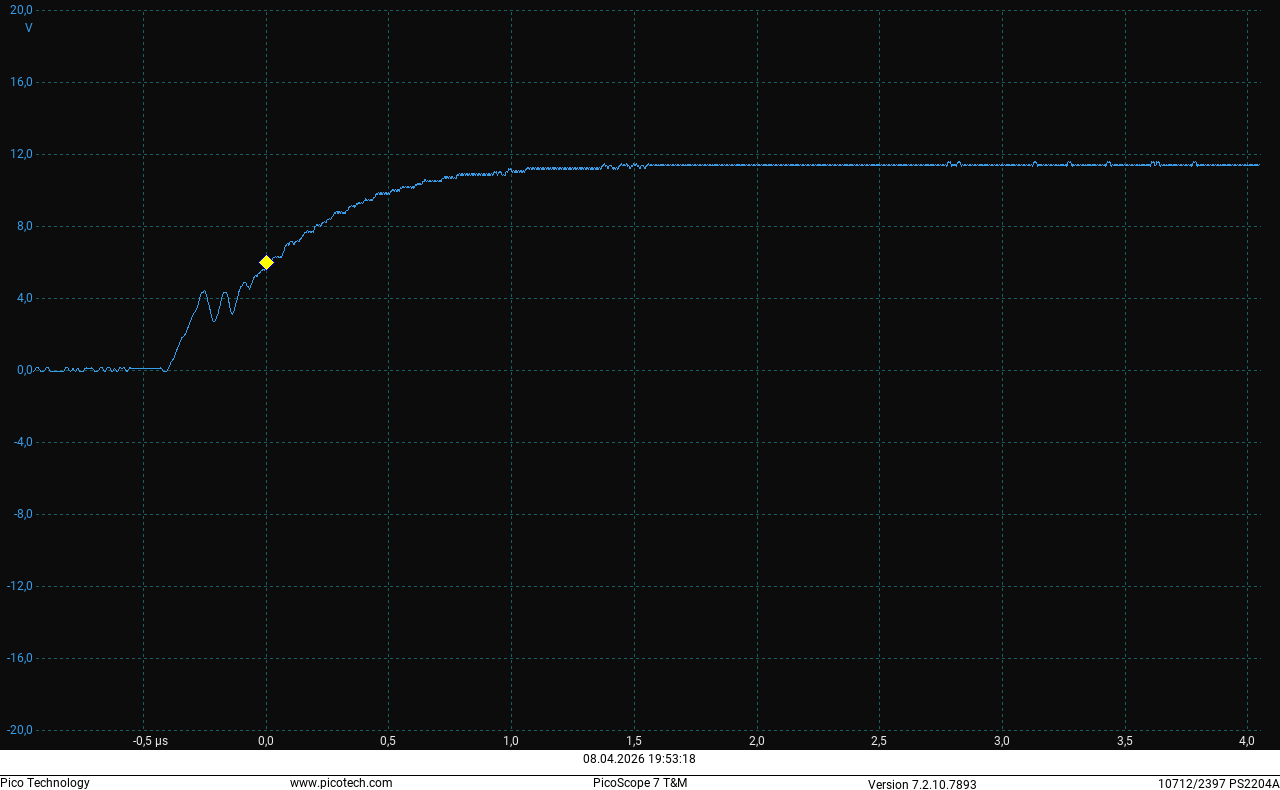
\includegraphics[width=0.99\textwidth, trim=0 40 0 0, clip]{images/leitend_oberschwinger.png}
    \caption{Schaltflanke des LS-Gates (Phase U) zur Validierung des Miller-Plateaus und des Gate-Widerstands. \\Zeitbasis: $0{,}5\,\mathrm{\mu s/div}$.}
    \label{fig:app_gate_flanke}
\end{figure}
\clearpage

\subsection{Zyklische Kommutierungszustände}
\label{app:cyclic}

\begin{figure}[H]
    \centering
    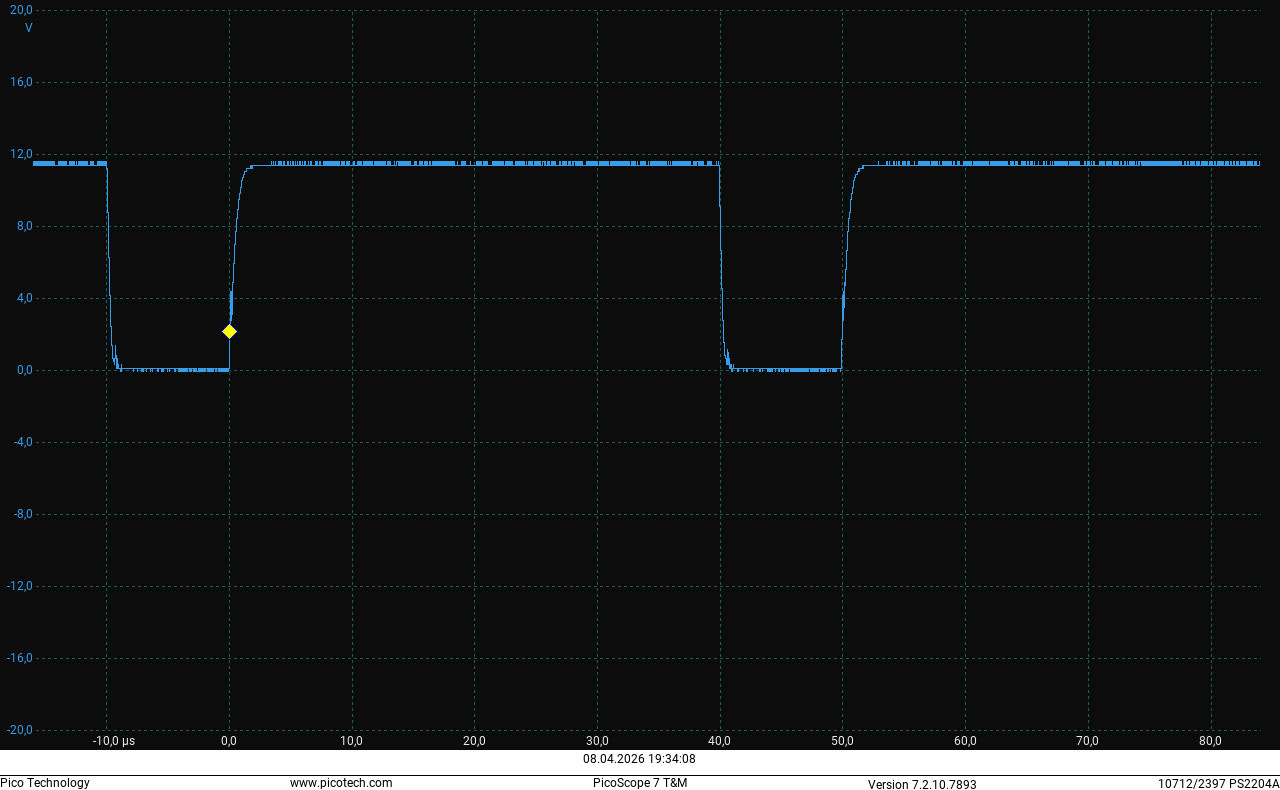
\includegraphics[width=0.99\textwidth, trim=0 40 0 0, clip]{images/Leitend.png}
    \caption{Aktiver Sektor (PWM mit $20\,\mathrm{kHz}$) mit Synchrongleichrichtung am LS-Gate. \\Zeitbasis: $10\,\mathrm{\mu s/div}$.}
    \label{fig:app_kommutierung_pwm}
\end{figure}

\begin{figure}[H]
    \centering
    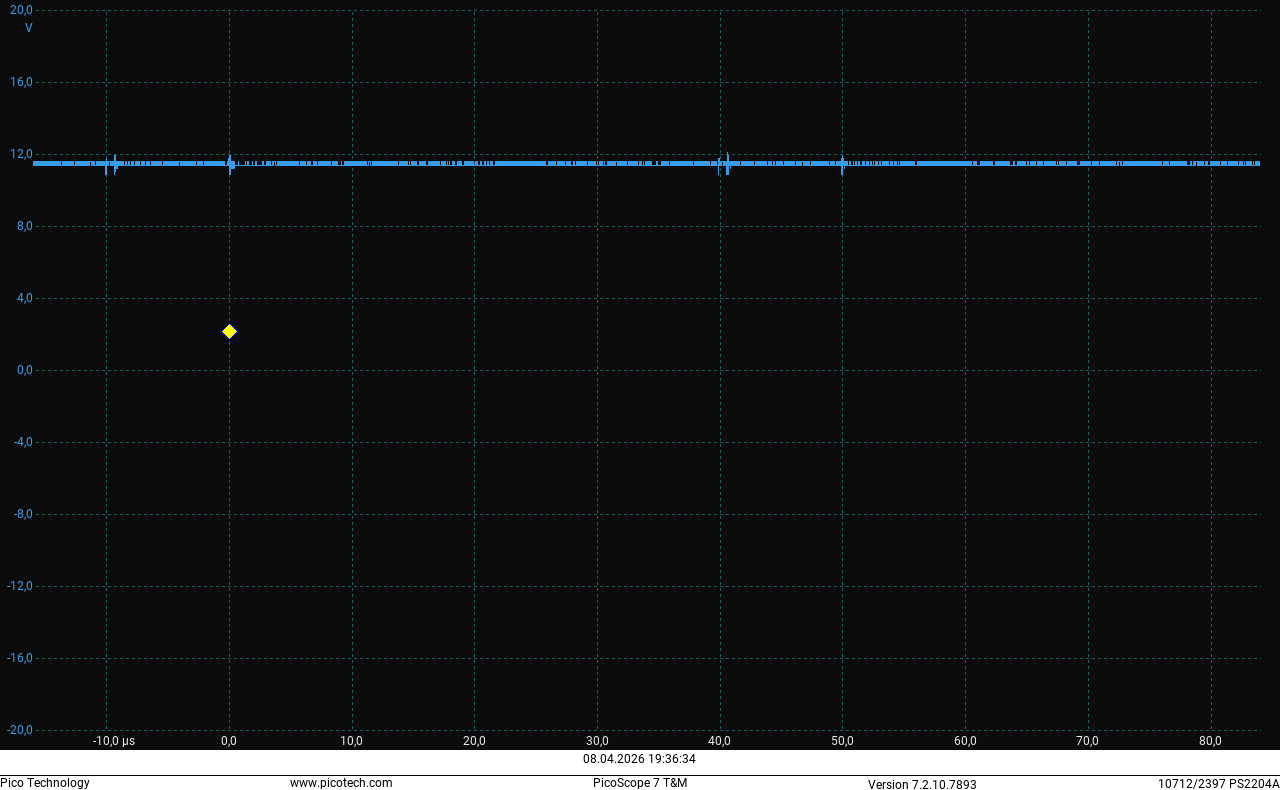
\includegraphics[width=0.99\textwidth, trim=0 40 0 0, clip]{images/full_leitend.png}
    \caption{Rückleiter-Betrieb mit statisch voll durchgesteuertem LS-Gate. \\ Zeitbasis: $10\,\mathrm{\mu s/div}$.}
    \label{fig:app_kommutierung_full}
\end{figure}

\begin{figure}[H]
    \centering
    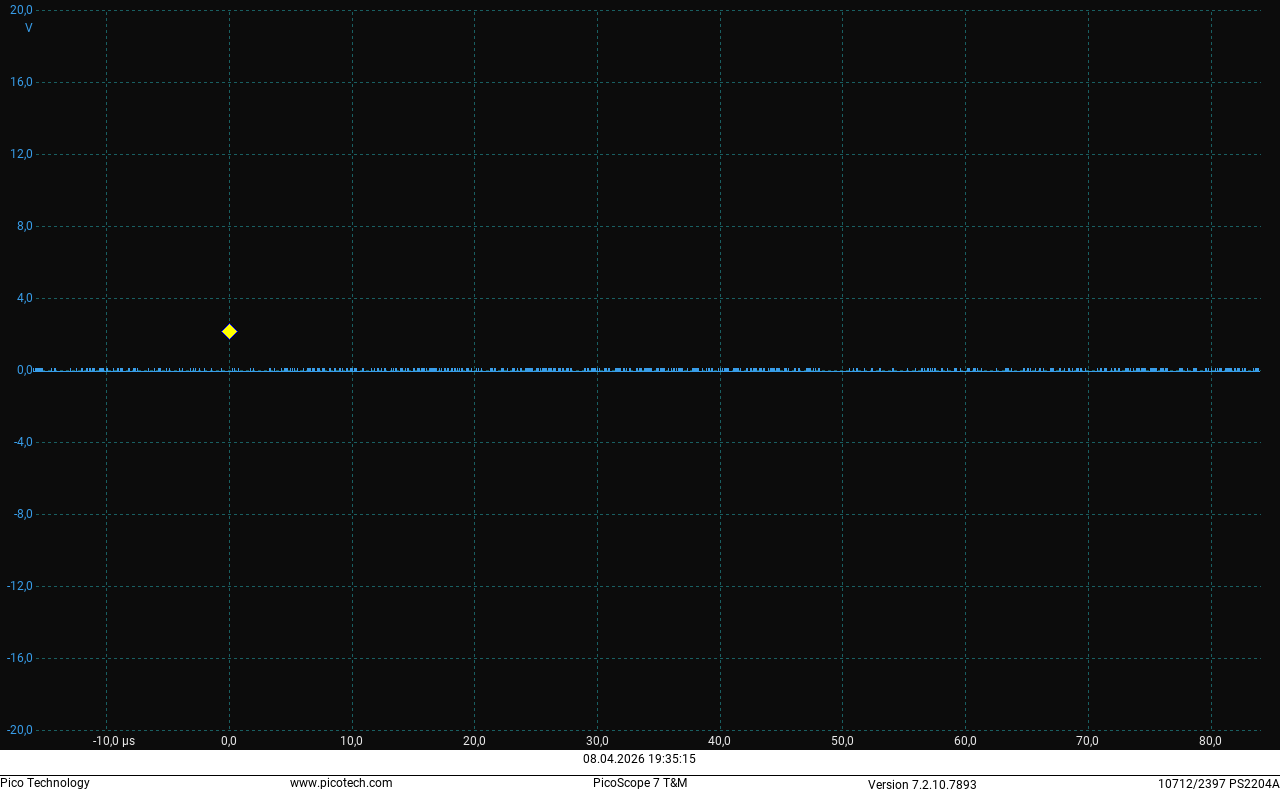
\includegraphics[width=0.99\textwidth, trim=0 40 0 0, clip]{images/floating.png}
    \caption{Floating-Betrieb mit hardwareseitig abgeschaltetem Gate. \\Zeitbasis: $10\,\mathrm{\mu s/div}$.}
    \label{fig:app_kommutierung_float}
\end{figure}